\documentclass{article}

\usepackage{url}
\usepackage{fancyhdr}
\usepackage{extramarks}
\usepackage{amsmath}
\usepackage{amsthm}
\usepackage{amsfonts}
\usepackage{tikz}
\usetikzlibrary{3d}
\usepackage[plain]{algorithm}
\usepackage{algpseudocode}
\usepackage{braket}
\usepackage{enumerate}
\usepackage{paralist}

%
% Basic Document Settings
%

\topmargin=-0.45in
\evensidemargin=0in
\oddsidemargin=0in
\textwidth=6.5in
\textheight=9.0in
\headsep=0.25in

\linespread{1.1}

\pagestyle{fancy}
\lhead{Habib University}
\chead{\hmwkClass, \hmwkTitle}
\rhead{\firstxmark}
\lfoot{\lastxmark}
\cfoot{\thepage}

\renewcommand\headrulewidth{0.4pt}
\renewcommand\footrulewidth{0.4pt}

\setlength\parindent{0pt}

%
% Create Problem Sections
%

\newcommand{\enterProblemHeader}[1]{
	\nobreak\extramarks{}{Problem \arabic{#1} continued on next page\ldots}\nobreak{}
	\nobreak\extramarks{Problem \arabic{#1} (continued)}{Problem \arabic{#1} continued on next page\ldots}\nobreak{}
}

\newcommand{\exitProblemHeader}[1]{
	\nobreak\extramarks{Problem \arabic{#1} (continued)}{Problem \arabic{#1} continued on next page\ldots}\nobreak{}
	\stepcounter{#1}
	\nobreak\extramarks{Problem \arabic{#1}}{}\nobreak{}
}

\setcounter{secnumdepth}{0}
\newcounter{partCounter}
\newcounter{homeworkProblemCounter}
\setcounter{homeworkProblemCounter}{1}
\nobreak\extramarks{Problem \arabic{homeworkProblemCounter}}{}\nobreak{}

%
% Homework Problem Environment
%
% This environment takes an optional argument. When given, it will adjust the
% problem counter. This is useful for when the problems given for your
% assignment aren't sequential. See the last 3 problems of this template for an
% example.
%
\newenvironment{homeworkProblem}[1][-1]{
	\ifnum#1>0
	\setcounter{homeworkProblemCounter}{#1}
	\fi
	\section{Problem \arabic{homeworkProblemCounter}}
	\setcounter{partCounter}{1}
	\enterProblemHeader{homeworkProblemCounter}
}{
	\exitProblemHeader{homeworkProblemCounter}
}

%
% Homework Details
%   - Title
%   - Due date
%   - Class
%   - Section/Time
%   - Instructor
%   - Author
%

\newcommand{\hmwkTitle}{Homework\ \#2}
\newcommand{\hmwkDueDate}{November 10, 2024, 11.59pm}
\newcommand{\hmwkClass}{CS 314/PHYS 300: Quantum Computing}
\newcommand{\hmwkClassInstructor}{Dr. Faisal Alvi}
\newcommand{\hmwkAuthorName}{\textbf{Student 1 Name, ID} \and \textbf{Student 2 Name, ID}}

%
% Title Page
%

\title{
	\vspace{2in}
	\textmd{\textbf{\hmwkClass:\\ \hmwkTitle}}\\
	\normalsize\vspace{0.1in}\small{\hmwkClassInstructor}\\
	\normalsize\vspace{0.1in}\small{Due\ on\ \hmwkDueDate}\\
	\vspace{3in}
}

\author{\hmwkAuthorName}
\date{}

\renewcommand{\part}[1]{\textbf{\large Part \Alph{partCounter}}\stepcounter{partCounter}\\}

%
% Various Helper Commands
%

% Useful for algorithms
\newcommand{\alg}[1]{\textsc{\bfseries \footnotesize #1}}

% For derivatives
\newcommand{\deriv}[1]{\frac{\mathrm{d}}{\mathrm{d}x} (#1)}

% For partial derivatives
\newcommand{\pderiv}[2]{\frac{\partial}{\partial #1} (#2)}

% Integral dx
\newcommand{\dx}{\mathrm{d}x}

% Alias for the Solution section header
\newcommand{\solution}{\textbf{\large Solution}}

% Probability commands: Expectation, Variance, Covariance, Bias
\newcommand{\E}{\mathrm{E}}
\newcommand{\Var}{\mathrm{Var}}
\newcommand{\Cov}{\mathrm{Cov}}
\newcommand{\Bias}{\mathrm{Bias}}

\begin{document}
	
\maketitle
	
\pagebreak
	
\begin{homeworkProblem}
(15 points) [\textbf{Measuring Bell States}] Given one of the following four bell states, i.e.
\begin{figure} [H]
 	\centering
 	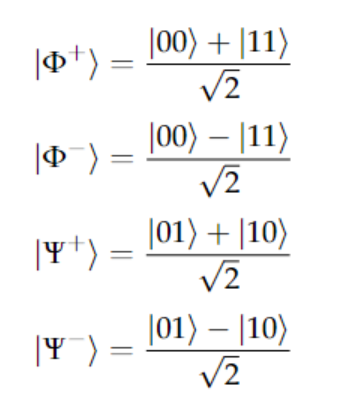
\includegraphics[scale = 0.7]{bell-states.png}
 	\caption{The Four Bell States $\ket{\phi^+}$, $\ket{\phi^-}$, $\ket{\psi^+}$, $\ket{\psi^-}$}
\end{figure}
		
\begin{enumerate}[(a)]
\item (5 points) Design a quantum circuit that measures the bell states, (i.e. perfectly distinguishes between each of the four bell states) with perfect probability.
\item (5 points) Show with analysis (for each of the four bell states) the output of the quantum circuit in (a).

\item (5 points) \textbf{Programming Component}

Write an implementation in Qiskit (Google Colab notebook is preferred) that implements the circuit in (a). Simulate the circuit for 1000 times for each of the four bell states and show the output as a histogram.  
\end{enumerate}
		

\end{homeworkProblem}
	
\begin{homeworkProblem} (25 points) [\textbf{Teleportation using GHZ like qubits}] This exercise develops (step-by-step) a teleportation protocol using GHZ like qubits.

\begin{enumerate}[(a)]
	
	\item (5 points) Design a quantum circuit that outputs the following state $\ket{\phi_{GHZlike}}$,
	\begin{equation}
		\ket{\phi_{GHZlike}} = \frac{1}{2} ( \ket{001} + \ket{010} + \ket{100} + \ket{111} ) \nonumber
	\end{equation}
	given the input qubits as $\ket{000}$.

	\item (5 points) Consider the following scenario where Alice wants to send an arbitrary qubit $\ket{\psi} = \alpha \ket{0} + \beta \ket{1}$ to Bob with the help of a facilitator Carlos.
	
	Show that the tensor product of the state $\ket{\psi}$ with the qubit $\ket{\phi_{GHZlike}}$ can be simplified to the following equation:
	
	\begin{eqnarray}
		\ket{\psi}  \otimes  \ket{\phi_{GHZlike}} = 
		\frac{1}{2\sqrt{2}} &(\ket{\phi^+} \otimes X\ket{\psi} + \ket{\phi^-} \otimes XZ \ket{\psi} + \ket{\psi^+} \otimes \ket{\psi} + \ket{\psi^-} \otimes Z \ket{\psi}) \ket{0} \nonumber \\	
		 + \frac{1}{2\sqrt{2}} &(\ket{\phi^+} \otimes \ket{\psi} + \ket{\phi^-} \otimes Z \ket{\psi} + \ket{\psi^+} \otimes X\ket{\psi} + \ket{\psi^-} \otimes XZ\ket{\psi}) \ket{1} \\ \nonumber
	\end{eqnarray}	
	   
	\item (5+5 = 10 points) Using the above simplification, our objective is to design a quantum teleportation protocol, similar to the Quantum Teleportation protocol studied in class. 
	
	Consider the following partial protocol. Note that these are steps with some missing components to be filled in by you in parts (i) and (ii): 
	
	Alice, Bob and Carlos each are in possession a single qubit. This qubit possessed by Alice, Bob and Carlos is entangled as $\ket{\phi_{GHZlike}}$. Furthermore, Alice also possesses the arbitrary qubit $\ket{\psi}$. The objective of this exercise is to design a protocol (and a circuit) that teleports $\ket{\psi}$ from Alice to Bob.
	
	(i) (5 points) Design a Quantum Circuit that teleports the qubit $\ket{\psi}$ from Alice to Bob with the help of Carlos. Note that, at the end of the protocol, Alice and Carlos measure their qubit(s) and send the result classically to Bob. Bob then applies some procedures to his qubit to recover $\ket{\psi}$. The objective of this part is to design and construct this circuit.  
	
	The tensor product of the Alice's arbitrary qubit $\ket{\psi}$ with the $\ket{\phi_{GHZlike}}$ is as given in (a) of this question.
	
	(ii) (5 points) What are some of the steps that Bob needs to take based on the measurements of Alice and Carlos in order for Alice's arbitrary qubit to be teleported to Bob? State the teleportation protocol. 

	\item (5 points) \textbf{Programming Component}
	
	Write an implementation in Qiskit (colab notebook preferred)  that implements the teleportation circuit stated above. Simulate the circuit for 1000 times for various inputs. 
\end{enumerate}

\end{homeworkProblem}

\begin{homeworkProblem}
	(5 points) [\textbf{Extending the Deutsch-Jozsa Algorithm}] For the Deutsch Jozsa Algorithm, we are given an input function $f: \Sigma^n \rightarrow \Sigma$ where $\Sigma = \{0, 1\}$ such that we have a promise, i.e., the function $f$ is either one of these two cases:
	\begin{itemize}
		\item the function $f$ for the first half of the input bits is zero and for the second half of the input bits is 1. An Example: Let's suppose $f$ is a function from $\Sigma^3 \rightarrow \Sigma$. Then $f(000) = f(001) = ... = f(011) = 0$ and $f(100) = f(101) = ... = f(111) = 1$. Note that the function is balanced.
		\item the \textbf{sum of the number of times} for which $f = 1$ in the first half of the input bits and the number of times for which $f = 0$ in the second half of the bits is $N/2$ where $N$ = $2^n$. An Example: Let's suppose $f$ is a function from $\Sigma^3 \rightarrow \Sigma$. Then $N = 2^3 = 8$, so $N/2 = 4$. An example of such a function is, let $f(000) = 1, f(001) = 0, f(010) = 1, f(011) = 1, f(100) = 1, f(101) = 0, f(110) = 1, f(111) = 1$. Now since, in the first half, there are three values (indices) for which $f = 1$, and in the second half there is only one value (index) for which $f = 0$, therefore $3 + 1 = 4 = 8/2 = N/2$. An example of a function satisfying the above requirement is a constant function, since for a constant function this sum will always be $N/2$.
	\end{itemize}
	Modify the Deutsch-Jozsa Algorithm to distinguish between these two cases. State clearly the modfications and construct the modified circuit.
	
	\bigskip
	
\end{homeworkProblem}

\textbf{Submission Guidelines:}
\begin{enumerate}
	\item Submit your solutions involving content, proofs, etc. as a latex pdf. 
	\item Submit the programming part as .ipynb files or as links to Google Colab pages. 
	\item Submit the entire HW as a zipped file.
\end{enumerate}

\end{document}

